This chapter provides a brief summary of the Dispersive Optical Model.
A few motivating concepts and definitions, sourced from the extensive treatments of \cite{MahzoonPhDThesis, MBTE},
are followed by an explicit parameterization of the optical potential used for the DOM fits of Chapter \ref{DOMResults}.
For all sectors of experimental data used in said fits, the formulae connecting the optical potential
to the scattering data are given. For detail on the development of the DOM formalism, the seminal
work of Mahaux and Sartor \cite{Mahaux1991} and a recent review \cite{Dickhoff2018} are recommended.
The goal here is not to provide the complete underpinnings of the theory, which are available in
numerous sources elsewhere, but to discuss how the terms of the potential are sensitive
to different sectors of experimental data.
In addition, several computational improvements to our implementation of the DOM, important for
expanding the reach of the fully non-local DOM of \cite{MahzoonPhDThesis} to all even-even systems,
are pointed out. In all cases, the notation used conforms to \cite{MBTE}, which also provides an
introduction to second quantization and historical background for relevant many-body concepts.

\section{The Single-Particle Propagator}
The central project of the Dispersive Optical Model (like any optical model) is
to understand how nucleons move about in a nuclear many-body system as parameterized by an optical
potential.
Specifically, we wish to know
how a nucleon with energy $E$ and quantum numbers $\alpha$
(position, momentum, spin, isospin, etc.) at time $t_{0}$ will be measured at a
later time $t$ with quantum numbers $\beta$ after interaction with the
potential. Given a
Hamiltonian that models this interaction, the Schr\"odinger equation
relates the Hamiltonian to the time evolution of this state:
\begin{equation} \label{SchrodingerEquation}
    i\hbar\frac{\partial}{\partial t}\ket{\alpha, t_{0}; t} = H\ket{\alpha, t_{0}; t}
\end{equation}

\noindent
where $\ket{\alpha, t_{0}; t}$ is the state at time $t$, given an initial state
$\ket{\alpha, t_{0}}$. Simple substitution into Eq. \ref{SchrodingerEquation} shows
that the initial state propagates in time according to:
\begin{equation}
    \ket{\alpha, t_{0}; t} = e^{-\frac{i}{\hbar}H(t-t_{0})}\ket{\alpha, t_{0}}
\end{equation}

\noindent
In position space, the wavefunction of the particle at a given time, $\psi(\bm{r},t)$,
is the sum of over all contributions from the propagation of the initial state up to that time,
a direct application of Huygens principle:
\begin{equation} \label{PropagatorDerivation}
    \begin{split}
        \psi(\bm{r},t) & = \braket{r|\alpha, t_{0}; t}\\
        & = \int d\bm{r}'
        \braket{\bm{r}|e^{-\frac{i}{\hbar}H(t-t_{0})}|\bm{r'}}\braket{\bm{r'}|\alpha,t_{0}}
    \end{split}
\end{equation}

\noindent
The integrand of Eq. \ref{PropagatorDerivation} is referred to as the
``single-particle propagator'', 
denoted $G(r, r'; t-t_{0})$ in the time domain,
as it determines how the wavefunction of a single particle
propagates over time. Crudely speaking, the propagator can be interpreted as the
probability that a given
initial state will evolve into a final state according to the wave equation.

To conduct practical scattering calculations, the energy-domain representation of the progapator
may be more useful than the time-domain representation. Applying a Fourier Transform to the propagator
(and omitting the intermediate algebraic steps) gives us the energy-domain representation,
and brings the mathematical structure of the propagator into focus:
\begin{equation} \label{PropagatorFT}
    \begin{split}
        G(\bm{r},\bm{r'};E) & = \int_{-\infty}^{\infty}d(t-t')e^\frac{i}{\hbar}E(t-t')G(\bm{r},\bm{r'}; t-t')\\
        & = \braket{0|a_{\bm{r}}\frac{1}{E-H+i\eta}a^{\dagger}_{\bm{r'}}|0}\\
        & = \braket{\bm{r} | \frac{1}{E-H+i\eta} | \bm{r'}}
    \end{split}
\end{equation}

\noindent
where $a_{\bm{r}}$ and $a^{\dagger}_{\bm{r}}$ represent the particle removal and
addition operators in
the second-quantization picture, respectively, and $\ket{0}$ is the vacuum state.
Equation \ref{PropagatorFT} contains the same information as Eq. \ref{PropagatorDerivation}: that
the wavefunction $\psi(\bm{r})$ is the sum of the weighted contributions from
all $\bm{r'}$ and the weights
are determined by the difference between the energy $E$ and the evaluation of
$H$ on each of the $\bm{r'}$
contributions. Of course, we need not privilege $\bm{r}$-space; $G$ can be written using any
suitable single-particle basis. For example, the momentum-space representation for a spinless,
non-interacting free particle of mass $m$ and momentum $\bm{k}$ reads:
\begin{equation} \label{PropagatorKSpace}
    G^{0}(\bm{k}, \bm{k'}; E) = \delta(\bm{k}-\bm{k'})\frac{1}{E-\frac{\hbar^{2}k^{2}}{2m} + i\eta}
\end{equation}

\noindent
If the independent-particle model was exact and the mean-field potential could be perfectly known,
calculating the propagation of nucleons through the nucleus would as simple as calculating
single-particle scattering off a potential well. Such a calculation involves little more than
a matrix inversion of the Hamiltonian in the denominator of Eq. \ref{PropagatorFT}.
Real nucleon-nucleus scattering involves the possibility of excitations in the nucleus from the 
incident
nucleon so that the wavefunction of the compound system may be
very different from the that of the nuclear ground state.
The single-particle propagator must include these possibilities as well.
The propagator from the $\ket{\alpha}$ state at time $t$ to the state $\ket{\beta}$ at a later time
$t'$ is:
\begin{equation} \label{ManyBodySPPropagator}
    G(\alpha, \beta; t, t') =
    -\frac{i}{\hbar}\braket{\Psi^{N}_{0}|\mathcal{T}
    [a_{\alpha_{H}}(t)a^{\dagger}_{\beta_{H}}(t')]|\Psi^{N}_{0}}
\end{equation}

\noindent
Here, $\ket{\Psi^{N}_{0}}$ is the normalized Heisenberg ground state for the N-particle system with
eigenvalue $E^{N}_{0}$:
\begin{equation} \label{NParticleGroundState}
    \hat{H}\ket{\Psi^{N}_{0}} = E^{N}_{0}\ket{\Psi^{N}_{0}}
\end{equation}

\noindent
The time-ordering operator $\mathcal{T}$\footnote ensures
that operators with later time appear to the left
of operators with earlier time, important for the perturbative treatment to follow.
\footnotetext
{
    The time-ordering operator $T$ is defined as:
    \begin{equation*}
        \mathcal{T}[a_{\alpha_{H}}(t)a^{\dagger}_{\beta_{H}}(t')]=\theta(t-t')a_{\alpha_{H}}(t)a^{\dagger}_{\beta_{H}}(t')
        -\theta(t'-t)a^{\dagger}_{\beta_{H}}(t')a_{\alpha_{H}}(t)
    \end{equation*}
}
In short, this expression includes contributions from both particle propagation, already seen 
Eq. \ref{PropagatorDerivation}, and hole propagation, new behavior only
pertinent for a many-particle system capable of excitation/hole production. We can expand Eq.
\ref{ManyBodySPPropagator} and once again apply a Fourier transform to make
interpretation easier:
\begin{equation} \label{LehmannRepresentation}
    \begin{split}
        G(\alpha,\beta;E) & =
        \int_{-\infty}^{\infty}d(t-t')e^{\frac{i}{\hbar}E(t-t')}G(\alpha,\beta;t-t')\\
        & = \sum_m
        \frac{\braket{\Psi^{N}_{0}|a_{\alpha}|\Psi^{N+1}_{m}}\braket{\Psi^{N+1}_{m}|a^{\dagger}_{\beta}|\Psi^{N}_{0}}}
        {E-(E^{N+1}_{m}-E^{N}_{0})+i\eta} +
        \frac{\braket{\Psi^{N}_{0}|a_{\beta}|\Psi^{N-1}_{n}}\braket{\Psi^{N-1}_{n}|a^{\dagger}_{\alpha}|\Psi^{N}_{0}}}
        {E-(E^{N}_{0}-E^{N-1}_{n})+i\eta}\\
        & =
        \braket{\Psi^{N}_{0}|a_{\alpha}\frac{1}{E-(\hat{H}-E_{0}^{N})+i\eta}a^{\dagger}_{\beta}|\Psi^{N}_{0}} +
        \braket{\Psi^{N}_{0}|a^{\dagger}_{\beta}\frac{1}{E-(E^{N}_{0}-\hat{H})-i\eta}a_{\alpha}|\Psi^{N}_{0}}
    \end{split}
\end{equation}

\noindent
$\ket{\Psi^{N\pm1}_{m(n)}}$ are the normalized Heisenberg states for the N$\pm$1 particle 
systems. The $\ket{\Psi^{N+1}_{m}}$ have eigenvalues $E^{N+1}_{m}$ and the
$\ket{\Psi^{N-1}_{n}}$ have 
eigenvalues $E^{N-1}_{n}$:
\begin{equation}
    \begin{split}
        \hat{H}\ket{\Psi^{N+1}_{m}} & = E^{N+1}_{m}\ket{\Psi^{N+1}_{m}}\\
        \hat{H}\ket{\Psi^{N-1}_{n}} & = E^{N-1}_{n}\ket{\Psi^{N-1}_{n}}
    \end{split}
\end{equation}

\noindent
in keeping with Eq. \ref{NParticleGroundState}. The second line
of Eq. \ref{LehmannRepresentation} is referred to as the ``Lehmann representation''.
To reach the third line of Eq. \ref{LehmannRepresentation}, the complete bases of
$\ket{\Psi^{N+1}_{m}}$ and $\ket{\Psi^{N-1}_{n}}$ have been removed from the first and second 
addends of the second line, respectively.
The particle and hole contributions to the propagator are neatly separated and
each possesses the relevant energy weighting in the denominator, sandwiched between the fermion 
creation and annihilation operators. Neither the ground-state wavefunction of the correlated
many-body system $\Psi^{N}_{0}$ or the full Hamiltonian $\hat{H}$ are known at this stage, but they
are now amenable to a perturbation expansion, the subject of the next section.

\subsection{Pertubation Expansion and The Dyson Equation}
The full single-particle propagator $G$ can be calculated via perturbation
expansion by starting with a non-interacting (unperturbed) propagator $G_{0}$
and adding interaction 
terms, $\hat{V}$, that bring $G_{0}$ closer to the real $G$. This expansion requires a change from
the Heisenberg picture of the previous section to the Interaction picture\footnote{Operators in the
    Interaction picture are related to those in the Schr\"odinger picture by:
    \begin{equation*}
        O_{I}(t) = e^{\frac{i}{\hbar}\hat{H}_{0}t}O_{S}e^{\frac{-i}{\hbar}\hat{H}_{0}t}
    \end{equation*}
    Appendix A of \cite{MBTE} provides a complete description of these different quantum-mechanical
pictures.}. First, the full Hamiltonian $H$ is broken up into the non-interacting and interacting
parts:
\begin{equation}
    \hat{H} = \hat{H_{0}}+\hat{H}_{1}
\end{equation}

\noindent
where $\hat{H_{0}}$ contains the kinetic energy operator $\hat{T}$ and possibly a one-body auxiliary
potential $\hat{U}$, and $\hat{H_{1}}$ collects all residual interactions (the hard part of the
problem). Broken up in this way, the non-interacting propagator reads:
\begin{equation}
    G^{(0)}(\alpha, \beta; t-t') =
    -\frac{i}{\hbar}\braket{\Phi^{A}_{0}|
    \mathcal{T}[a_{\alpha I}(t)a^{\dagger}_{\beta I}(t')]|\Phi^{A}_{0}}
\end{equation}

\noindent
where the fully-correlated many-body ground state $\ket{\Psi^{A}_{0}}$ has been replaced by
$\ket{\Psi^{A}_{0}}$, the uncorrelated ground-state associated with $H_{0}$. Through algebraic
manipulation and employing the Interaction version of all operators,
the \textit{full} single-particle propagator, including the
contribution from the interactions buried in $\hat{H_{1}}$, is:
\begin{equation} \label{FullSPPropagator}
    G(\alpha, \beta; t-t') = \frac{Num}{Denom}
\end{equation}

\noindent
where
\begin{equation*}
    \begin{split}
        Num & = -\frac{i}{\hbar}\sum^{\infty}_{n}\left(\frac{i}{\hbar}\right)^{n}\frac{1}{n!}
    \int_{-\infty(1-i\eta)}^{\infty(1-i\eta)} dt_{1}
    \int_{-\infty(1-i\eta)}^{\infty(1-i\eta)} dt_{2} \cdots
    \int_{-\infty(1-i\eta)}^{\infty(1-i\eta)} dt_{n}\\
    & \phantom{ {}= } \times \braket{\Phi^{N}_{0}|\mathcal{T}[\hat{H}_{1}(t_{1})
    \hat{H}_{1}(t_{2}) \cdots \hat{H}_{1}(t_{n})a_{\alpha I}(t)a^{\dagger}_{\beta
    I}(t')]|\Phi^{N}_{0}}\\\\
    Denom & = \sum^{\infty}_{m}\left(\frac{-i}{\hbar}\right)^{m}\frac{1}{m!}
        \int_{-\infty(1-i\eta)}^{\infty(1-i\eta)} dt'_{1}
        \int_{-\infty(1-i\eta)}^{\infty(1-i\eta)} dt'_{2} \cdots
        \int_{-\infty(1-i\eta)}^{\infty(1-i\eta)} dt'_{m}\\
        & \phantom{ {}= } \times \braket{\Phi^{N}_{0}|
        \mathcal{T}[\hat{H}_{1}(t_{1})
        \hat{H}_{1}(t_{2}) \cdots \hat{H}_{1}(t_{m})(t')]|\Phi^{N}_{0}}
    \end{split}
\end{equation*}

\noindent
Despite the extra ink, the mathematical structure of the Lehmann
representation (Eq. \ref{LehmannRepresentation}) is still visible: the numerator contains
the contributions from the creation and annihilation operators attaching to the uncorrelated
ground-state, and the denominator provides an energy weighting. We have generated an infinite
series of terms with increasing order in the number of $\hat{H}_{1}$ interactions permitted.
Aside from arbitrary counting indices,
the only differences between the numerator and denominator are a
factor of $-\frac{i}{\hbar}$ and the fermion annihilation and creation operators
responsible for moving from $\ket{\alpha}$ to $\ket{\beta}$. Wick's
theorem\footnote{See section 8.4 of \cite{MBTE}
for the full procedure.} can be applied to remove contributions to the propagator
that appear in both the numerator and the denominator and do not survive the
division. This dramatically
reduces the number of terms at each level of the perturbation expansion, and when the dust settles,
the propagator reads:
\begin{equation} \label{ManyBodySPPropagatorConnected}
    \begin{split}
    G(\alpha, \beta; t-t') & =
    -\frac{i}{\hbar}\sum^{\infty}_{n}(\frac{i}{\hbar})^{n}
    \frac{1}{n!}\int dt_{1} \int dt_{2} \cdots \int dt_{n}\\
    & \phantom{ {}= } \times \braket{\Phi^{A}_{0}|
    \mathcal{T}[\hat{H}_{1}(t_{1})
    \hat{H}_{1}(t_{2}) \cdots \hat{H}_{1}(t_{n})a_{{\alpha}I}(t)a^{\dagger}_{{\beta}I}(t')]|\Phi^{A}_{0}}_{connected}
\end{split}
\end{equation}

Physically speaking, the full propagator is the infinite sum of the expectation value of 
an $\hat{H_{1}}$ iteratively applied to the non-interacting ground state. The
non-interacting ground state is modified by each interaction and thus all the many-body correlations
of $\ket{\Psi^{N}_{0}}$ are encoded by the repeated operation of $\hat{H_{1}}$. The subscript
``connected'' indicates that the only terms that survive correspond to fully-connected Feynman 
diagrams, as all non-connected diagrams appear in both the numerator and denominator of Eq. 
\ref{FullSPPropagator}.

We can represent the perturbation expansion of Eq. \ref{ManyBodySPPropagatorConnected}
diagrammatically to clarify the physical meaning of the expansion terms. Figure
\ref{PerturbationExpansionDiagram} shows several diagrams from the first few orders of the
expansion. To zeroth-order, 
the expansion is only one purely non-interacting term, which is just the free single-particle 
propagator. At each higher order, one more interaction is permitted to enter the diagram at any
fermion line (i.e., into any propagator line). By grouping and rearranging the terms, we can 
condense the full perturbation expansion to a
self-consistent equation called the Dyson equation:
\begin{equation} \label{DysonEquation}
    G(\alpha,\beta;E) = G^{(0)}(\alpha,\beta;E) +
    \sum_{\gamma,\delta}G^{(0)}(\alpha,\gamma;E)\Sigma^{*}(\gamma,\delta,E)G(\delta, \beta; E)
\end{equation}

\noindent
A diagrammatic representation of the Dyson equation is given in Fig. \ref{DysonEquationDiagram}.
\begin{figure}[ht!]
    \centering
    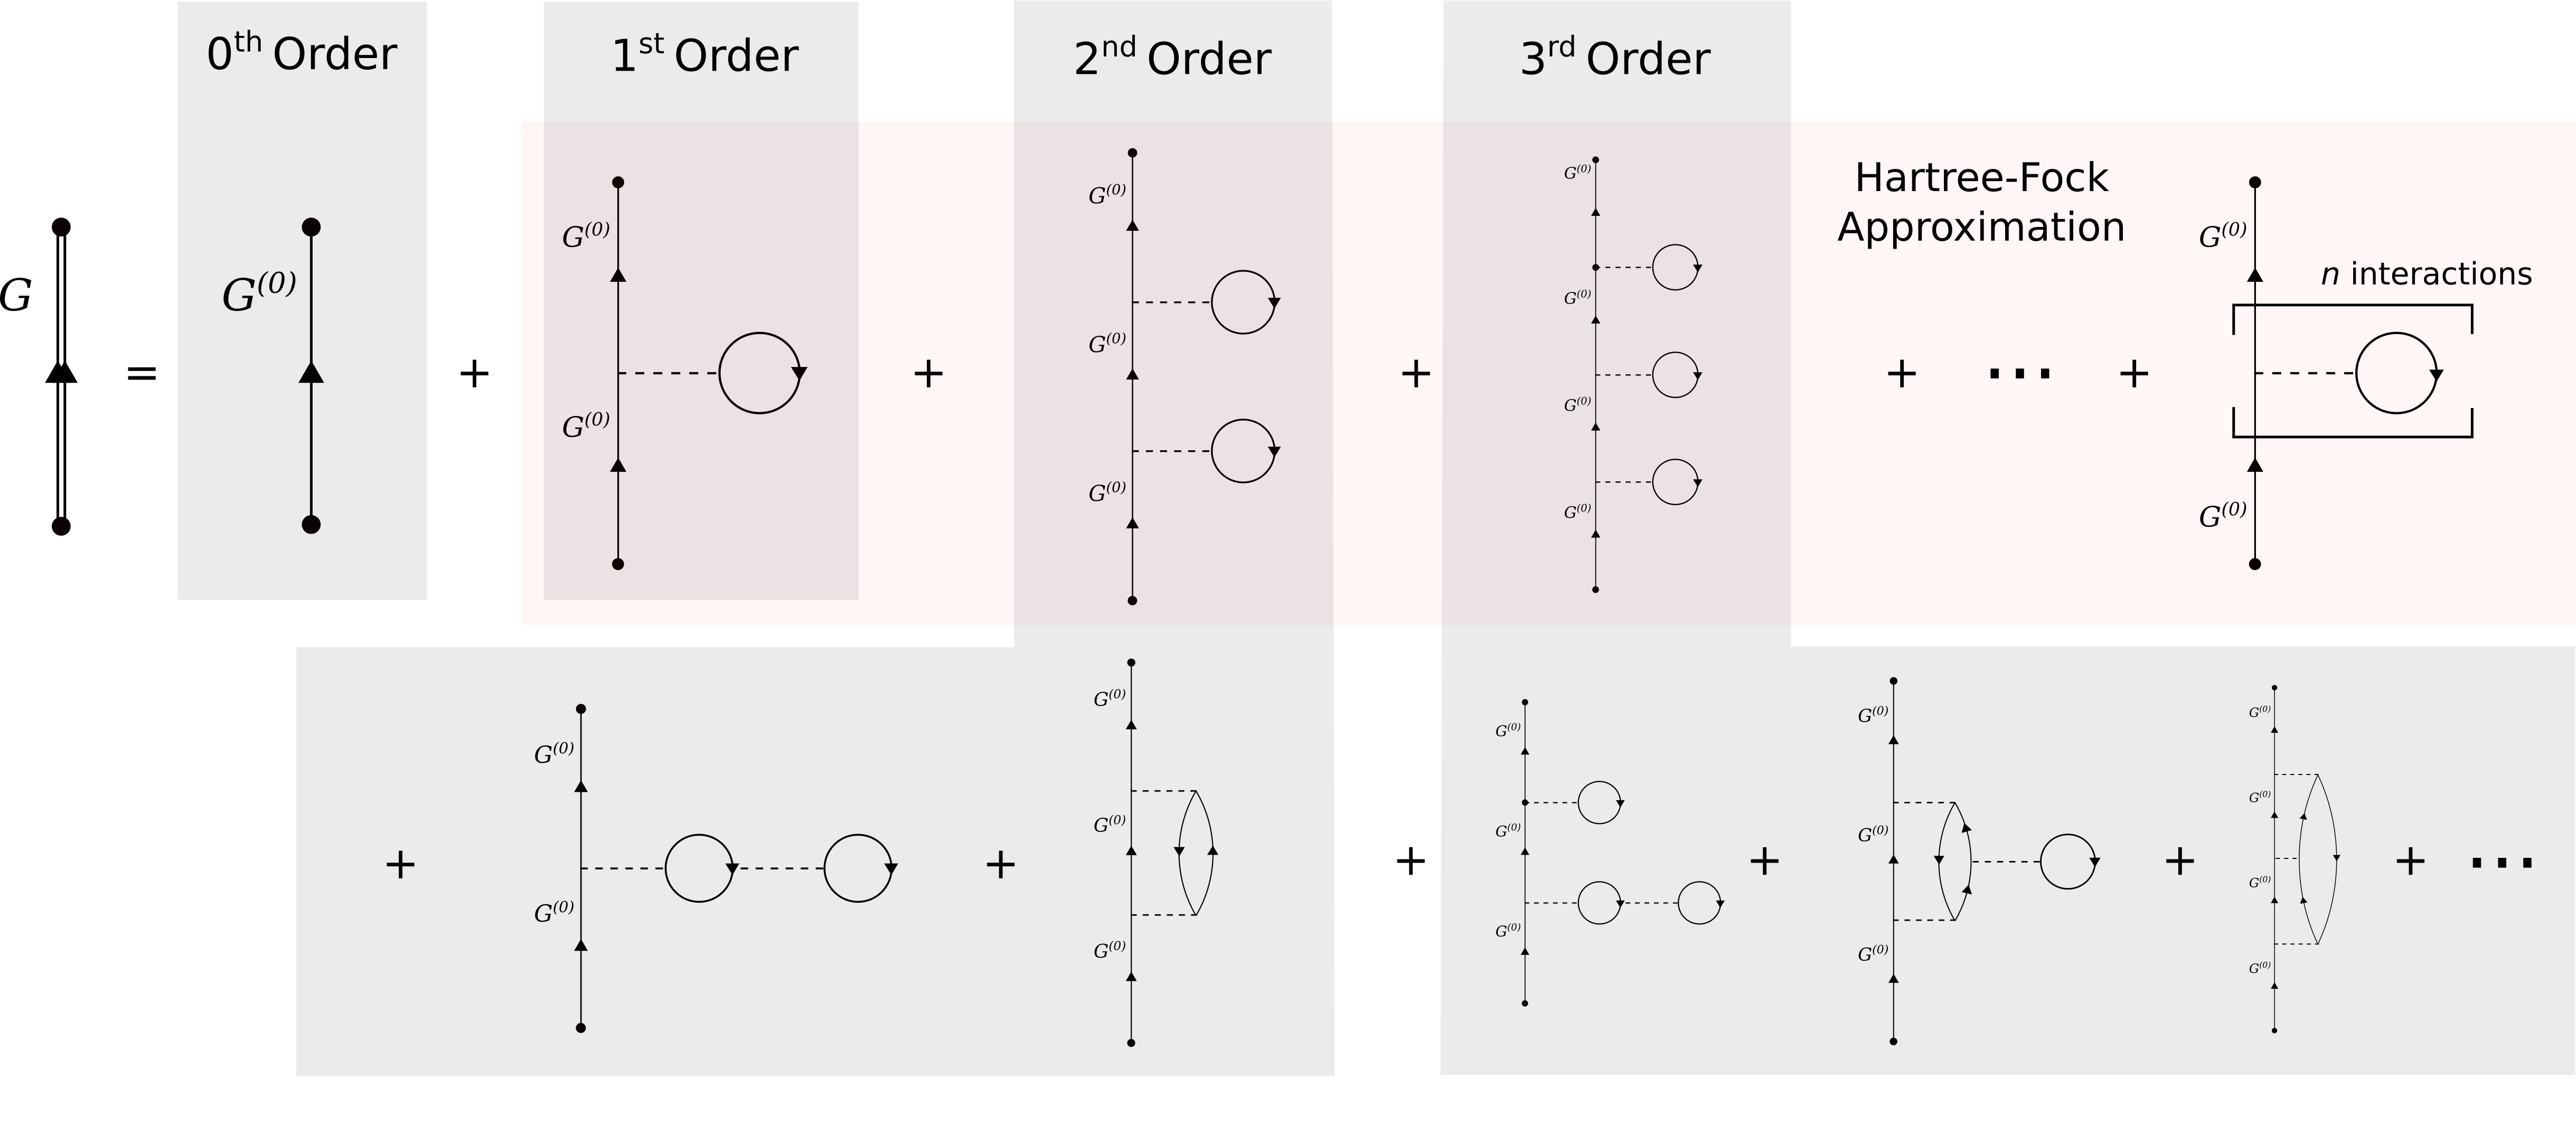
\includegraphics[width=0.9\textwidth]{figures/SecondOrder.png}
    \caption[The single-particle propagator perturbation expansion, to second order]
    {
        Example diagrams from the first few orders of the 
        single-particle propagator perturbation expansion.
        The interaction $\hat{V}$ is indicated by the horizontal
        dashed line and is taken to be two-body only in this treatment.
        The terms of each order are grouped by gray boxes and terms that contribute to
        the Hartree-Fock approximation are surrounded by the red box. In each Hartree-Fock
        term, the particle interacts with the mean-field of the nucleus but
        the nucleus is never excited and thus the interaction has no energy dependence.
    }
    \label{PerturbationExpansionDiagram}
\end{figure}

\begin{figure}[ht!]
    \centering
    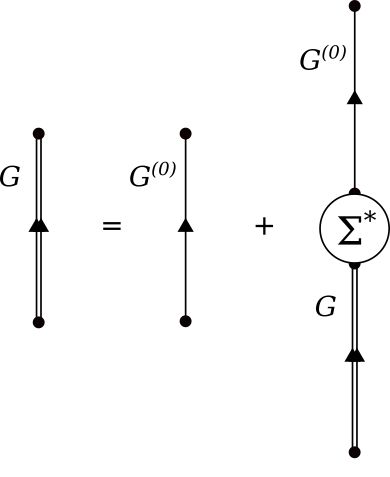
\includegraphics[width=0.4\textwidth]{figures/DysonEquation.png}
    \caption{The Dyson equation in diagrammatic form.}
    \label{DysonEquationDiagram}
\end{figure}

The summation variables $\gamma$ and $\delta$ label states internal to the diagrams that are 
accessed during the particle's excitation of the many-body system\footnotemark.
\footnotetext
{
    If a three-body interaction was included in $\hat{H}_{0}$, additional labels would be needed.
}
The Dyson
equation introduces a new term, the irreducible self-energy $\Sigma^{*}$, that connects the free
single-particle propagator to the full single-particle propagator that incorporates all the
in-medium effects of traveling through the nuclear environment. The self-energy serves the role
of the potential - the optical potential - experienced by a particle in the medium.
This makes the Dyson equation the
equivalent of the Schr\"odinger equation, but for particles \textit{embedded in the medium} 
rather than propagating in free space. Calculating the full self-energy explicitly remains
impossible in practice,
as it involves a (countably) infinite number of diagrams and the underlying nuclear
interactions are only approximately known. Rather than solve this problem
analytically, the DOM solves it empirically by identifying the full self-energy as equivalent
to the optical potential. By fitting the self-energy to experimental data, we
cut the Gordian knot of making an analytic calculation to all orders.
As already discussed in Chapter \ref{introduction}, the optical potential is  
readily connected to a host of experimental data: elastic cross sections, analyzing powers, and 
inelastic reactions for both protons and neutrons.
From a well-constrained optical-potential/self-energy, additional important quantities, like
overlap functions and neutron skins, can be extracted. This phenomenological approach is the 
heart of the Dispersive Optical Model.

\subsection{The Dispersion Relation}
State-of-the-art optical models \cite{CH89, KoningDelaroche} typically
restrict their potentials to the
positive-energy domain relevant for nucleon-nucleus scattering. From the previous
section, though, it is clear that the self-energy must have a negative-energy component
if it is to describe the
correlated many-body ground state: bound nucleons experience the same potential
as scattering nucleons, albeit at negative energies.
It has been recognized for over fifty years \cite{FeshbachDispersionRelation,
Passatore1967} that because the optical potential is a complex function, the real and imaginary
parts should obey a dispersion relation: if the real part is known at all energies (positive and
negative), the imaginary part can be deduced and vice-versa. Optical models that obey this relation
may be called dispersive optical models.

The real part of the self-energy can be shown to have two components: one independent of energy
(equal to the correlated Hartree-Fock term)
and an energy-dependent part that can be calculated from the imaginary part:
\begin{equation} \label{RealPart}
    \operatorname{Re}(\Sigma^{*}(\alpha,\beta; E)) =
    \operatorname{Re}(\Sigma_{s}(\alpha,\beta)) +
    \operatorname{Re}({\Sigma_{d}(\alpha,\beta; E)})
\end{equation}

\noindent
The relevant dispersion relation to calculate the real energy-dependent part is:
\begin{equation} \label{DispersionRelation}
    \operatorname{Re}({\Sigma_{d}(\alpha,\beta; E)}) =
    -\mathcal{P}\int_{\epsilon^{+}_{T}}^{\infty}\frac{dE'}{\pi}
    \frac{\operatorname{Im}({\Sigma_{d}(\alpha,\beta; E')})}{E-E'}
    + \mathcal{P} \int_{-\infty}^{\epsilon^{-}_{T}}\frac{dE'}{\pi}
    \frac{\operatorname{Im}({\Sigma_{d}(\alpha,\beta; E')})}{E-E'}
\end{equation}

\noindent
$\mathcal{P}$ is the Cauchy principle value and the integration limits $\epsilon^{\pm}_{T}$ are
selected to be just below the lowest-lying imaginary strength in the positive-energy domain
(for $\epsilon^{+}_{T}$) and just above the highest-lying imaginary strength in the negative-energy
domain (for $\epsilon^{-}_{T}$). Between these thresholds, the imaginary component of the potential
vanishes, so the self-energy is entirely real. After some algebraic rearrangement,
it can be shown that:
\begin{equation} \label{SubtractedDispersionRelation}
    \begin{split}
        \operatorname{Re}({\Sigma(\alpha,\beta; E)}) =
        & \operatorname{Re}({\Sigma(\alpha,\beta;\epsilon_{F})})\\
        & -\mathcal{P}\int_{\epsilon^{+}_{T}}^{\infty}\frac{dE'}{\pi}
        \frac{\operatorname{Im}({\Sigma_{d}(\alpha,\beta; E')})}{E-E'}
        \left[\frac{1}{E-E'}-\frac{1}{\epsilon_{F}-E'}\right]\\
        & + \mathcal{P} \int_{-infty}^{\epsilon^{-}_{T}}\frac{dE'}{\pi}
        \frac{\operatorname{Im}({\Sigma_{d}(\alpha,\beta; E')})}{E-E'}
        \left[\frac{1}{E-E'}-\frac{1}{\epsilon_{F}-E'}\right]
    \end{split}
\end{equation}

\noindent
which is referred to as the ``subtracted dispersion relation''. The integral of the imaginary
component of the self-energy over the entire energy domain determines the dynamic (energy-dependent)
part of the real component, ensuring that the potential is self-consistent and that reactions and
structure calculations take place on equal footing. This is the form of the dispersion relation
employed in the subsequent analysis.

\section{Connection to Experimental Observables}

\subsection{Elastic and inelastic nucleon scattering}
For nucleon-nucleus scattering, the momentum basis is a natural choice. The scattering amplitude can be directly calculated using the
reducible self-energy $\Sigma$\footnotemark:
\footnotetext
{
    The reducible self-energy is related to the irreducible
    self-energy of Eq. \ref{DysonEquation} by:
    \begin{equation}
        \Sigma = \Sigma^{*} + \Sigma^{*}G^{(0)}\Sigma
    \end{equation}. See \cite{MahzoonPhDThesis} for details.
}
\begin{equation}
    f_{m'_{s},m_{s}}(\theta,\phi) =
    -\frac{4m\pi^{2}}{\hbar^{2}}\braket{\bm{k}'m'_{s}|\Sigma(E)|\bm{k}m_{s}}
\end{equation}

\noindent
where $\bm{k}m_{s}$ are the wave vector and spin quantum number of the incident nucleon and
$\bm{k'}m'_{s}$ are for the exiting nucleon. The matrix structure of the right side can be
split into spin-independent and spin-dependent portions $\mathcal{F}$ and $\mathcal{G}$:
\begin{equation}
    f(\theta,\phi) = \mathcal{F}(\theta)I + \sigma\cdot\bm{\hat{n}}\mathcal{G}(\theta)
\end{equation}

\noindent
where
\begin{equation}
    \begin{split}
        \mathcal{F}(\theta) & = \frac{1}{2ik}\sum_{l=0}^{\infty}\left[(l+1)e^{2i\delta_{l+} - 1} +
        l\left(e^{2i\delta_{l-}}-1\right)\right]P_{l}(cos\theta)\\
        \mathcal{G}(\theta) & =
        \sigma\cdot\bm{\hat{n}}\left[\frac{sin\theta}{2k}\sum_{l=1}^{\infty}[e^{2i\delta_{l+}}-e^{2i\delta_{l-}}]P'_{l}(cos\theta)\right]
    \end{split}
\end{equation}

\noindent
Here, $P_{l}$ are Legendre polynomials of degree $l$, $P_{l}'$ is the derivative of the Legendre
polynomial, and $\delta_{l\pm} \equiv \delta_{l\pm\frac{1}{2}}$, corresponding to the spin being
parallel or antiparallel to the orbital angular momentum.

\noindent
From the scattering amplitude, the unpolarized cross section is simply:
\begin{equation}
    \left(\frac{d\sigma}{d\Omega}\right)(\theta) = |\mathcal{F}(\theta)|^{2}
    +|\mathcal{G}(\theta)|^{2}
\end{equation}

\noindent
and the analyzing power is:
\begin{equation}
    A(\theta) = \frac{2\mathcal{F}(\theta)(\mathcal{G}(\theta))^{*}}
    {\frac{d\sigma}{d\Omega}(\theta)}
\end{equation}

\noindent
The complex phase shift (equivalently, the S-matrix elements) for each partial wave associated
with the nucleon under investigation can be
calculated directly from the reducible self-energy:
\begin{equation}
    \begin{split}
        e^{2i\delta_{lj}} & \equiv \braket{\bm{k}|\mathcal{S}_{lj}(E)|\bm{k}}\\
        & = 1 - 2\pi i \left(\frac{mk}{\hbar^{2}}\right) \braket{\bm{k}|\Sigma_{lj}(E)|\bm{k}}
    \end{split}
\end{equation}

\noindent
where $k$ is the center-of-mass momentum of the nucleon, $m$ is the nucleon mass, and $E$ is the
center-of-mass energy. The reaction cross section at a given energy is the sum of the partial
reaction cross section over all partial waves:
\begin{equation}
    \sigma_{rxn} = \sum^{\infty}_{l=0}\frac{\pi}{k^{2}}
    \left[(2l+1)-(l+1)|e^{2i\delta_{l+}}|^{2}-l|e^{2i\delta_{l-}}|^{2}\right]
\end{equation}

\noindent
and the total cross section simply a sum of the reaction and elastic of all partial waves:
\begin{equation}
    \sigma_{tot} = \sigma_{el} + \sigma_{rxn}\\
\end{equation}

\noindent
where
\begin{equation}
    \begin{split}
        \sigma_{el} & = \int d\theta \int d\phi\ \frac{d\sigma}{d\Omega}(\theta)\\
        & = \sum^{\infty}_{l=0}\frac{\pi}{k^{2}}
        \frac{|(l+1)(e^{2i\delta_{l+}}-1)+l(e^{2i\delta_{l-}}-1)|^{2}}{2l+1}\\
        & \times \frac{l(l+1)|e^{2i\delta_{l+}}-e^{2i\delta_{l-}}|^{2}}{2l+1}
    \end{split}
\end{equation}

\subsection{Bound-state properties}
To compare the bound-state information of the propagator with experimental data, we first
define the spectral functions for holes and particles:
\begin{equation}
    \begin{split}
        S_{h}(\alpha; E) & =
        \frac{1}{\pi}\operatorname{Im}({G(\alpha,\alpha;E)})\qquad \text{for } E\leq\epsilon_{F}^{-}\\
        & = \sum|\braket{\Psi^{N-1}_{n}|a_{\alpha}|\Psi^{N}_{0}}|^{2}
        \delta(E-(E^{N}_{0}-E_{n}^{N-1}))\\
        \\
        S_{p}(\alpha; E) & =
        -\frac{1}{\pi}\operatorname{Im}({G(\alpha,\alpha;E)})\qquad \text{for } E\geq\epsilon_{F}^{+}\\
        & = \sum|\braket{\Psi^{N+1}_{n}|a_{\alpha}^{\dagger}|\Psi^{N}_{0}}|^{2}
        \delta(E-(E_{n}^{N+1}-E^{N}_{0}))
    \end{split}
\end{equation}
\noindent
In this expression, $\epsilon_{F}^{\pm}$ are the lowest-unoccupied and highest-occupied
single-particle levels, which yield the Fermi energy $\epsilon_{F}$ when averaged. Physical
speaking, the hole spectral function at the energy E is the probability density for plucking out
a particle with quantum numbers $\alpha$ from the ground state and leaving the residual nucleus with the
energy $E^{N}_{0}-E$. The particle spectral function provides the same information, but for adding a
particle instead, leaving the nuclear system with energy $E^{N}_{0}+E$. From the spectral functions, the occupation of a state is simply
\begin{equation} \label{ParticleNumber}
    \begin{split}
        n(\alpha) & = \braket{\Psi^{N}_{0}|a_{\alpha}^{\dagger}a_{\alpha}|\Psi^{N}_{0}}\\
        & = \int_{-\infty}^{-\epsilon_{F}}S_{h}(\alpha; E)
    \end{split}
\end{equation}

\noindent
Numerically, this integral can be difficult to compute near $\epsilon_{F}$ where peaks in the
spectral function (from bound quasi-hole states just below $\epsilon_{F}$) become $\delta$-function-like. 
This is a consequence of the vanishing imaginary strength near $\epsilon_{F}$. Thus, we use a piecemeal procedure
where the spectral function is integrated up to an arbitrary threshold near (but below) the
$\delta$-function-like behavior, and the spectroscopic factor of any quasi-holes between the threshold and
$\epsilon_{F}^{-}$ is added to account for the remaining occupation. The spectroscopic factor is
calculated:
\begin{equation}
    [insert SF calculation]
\end{equation}

Previous DOM analyses (e.g., \cite{MahzoonPhDThesis}) dealt only with doubly-closed 
shell nuclei such as \caForty\ and \caEight.
For these nuclei, the above procedure to calculate the occupation number is
sufficient. The present analysis includes nuclei with open neutron subshells
(e.g., the $\nu$ 0\dFive\ in \oEight\ and $\nu$ 0\fFive\ in \niEight), motivating a new
procedure. Per standard treatments of nucleon pairing \cite{BohrAndMottleson}, an additional
pairing parameter $\Delta$ was added to account for open subshells' fractional occupation $n_{\pm}$.
This parameter splits these subshells' occupants into upper and lower sublevels with energies 
$E_{\pm}$:
\begin{equation}
    E_{\pm} = \mu \pm ((\epsilon_{F}-\mu)^{2} + \Delta^{2})^{\frac{1}{2}}
\end{equation}

\noindent
where $\mu$ is the energy of the open subshell before pairing is considered and
$\epsilon_{F}$ is the Fermi
energy. The magnitude of $\Delta$ corresponds to the energy difference between
adding/removing a nucleon to/from that subshell. The subshell
is split between the upper and lower sublevels. The occupancy of these sublevels is calculated via:
\begin{equation}
    n_{\pm} = \frac{1}{2}\left( 1-\frac{\chi}{E_{\pm}}\right)
\end{equation}

\noindent
where $\chi = |E_{\pm}-\mu| - (\epsilon_{F} - \mu)$. Only occupation in the
lower sublevel is counted toward the total particle number. For each open-shell
nucleus with neutron number $N$ and proton number $Z$, $\Delta$ was fixed according to:
\begin{equation}
    \Delta(N,Z) = \frac{1}{4}\left(B(N-2,Z)-3B(N-1,Z) + 3B(N,Z)-B(N+1,Z)\right)
\end{equation}
\noindent
where $B(N,Z)$ is the nuclear binding energy.

In addition to the total occupation of each state with quantum numbers $\alpha$,
the density distribution of particles in that state in r-space can be calculated. By summing the
single-particle position-space distributions, the total point distributions for
protons and neutrons can be calculated.
After folding this distribution with an appropriate form factor giving the internal charge density
distribution for protons and neutrons \cite{FormFactorPaper}, the final distribution can be compared
to the experimental charge density distribution calculated in (e,e) scattering experiments.

The total binding energy of the nucleus may be calculated directly from the spectral function and the
kinetic energy operator $\hat{T}$:
\begin{equation} \label{TotalEnergyEquation}
    \begin{split}
        E^{N}_{0} & = \braket{\Psi^{N}_{0}|\hat{H}|\Psi^{N}_{0}}\\
        & = \frac{1}{2} \left(\sum_{\alpha,\beta}\braket{\alpha|\hat{T}|\beta}n_{\alpha,\beta}
        + \sum_{\alpha}\int_{-\infty}^{\epsilon_{F}^{-}}dE\ E\ S_{h}(\alpha;E)\right)
    \end{split}
\end{equation}

\noindent
and the discrete single-particle energy levels can be calculated by diagonalizing the
Hamiltonian.

\section{Parameterization of the Potential}
The functions used to parameterize the optical potential
are selected to conform with general physical intuition about the nuclear
many-body problem and past experience with optical potentials. Accordingly,
the self-energy should be, non-local, complex, and dispersively correct.
Before detailing the full parameterization,
a few standard mathematical forms need to be introduced. In this section, the free variables that
are fitted to data during the DOM procedure are denoted in a bold typeface. In the basic functional
forms of the next subsection, these variables are not labeled with numbers,
but in the following subsections, the bolded
variables are assigned numbers to facilitate comparison with the
list of parameter values of Appendix \ref{DOMParameters}.

\subsection{Functional forms}
We use two standard form factors
to describe the radial dependence of components
associated with the nuclear volume (a Woods-Saxon shape)
and the nuclear surface (a derivative of the Woods-Saxon shape):
\begin{equation} \label{WoodsSaxon}
    \begin{split}
        f_{vol}(r; \bm{R}, \bm{a}) & = \frac{-1}{1+e^{(r-\bm{R})/\bm{a}}}\\
        f_{sur}(r; \bm{R}, \bm{a}) & = \frac{1}{r}\frac{d}{dr}f_{vol}(r; \bm{R}, \bm{a})
    \end{split}
\end{equation}

\noindent
$\bm{R}$ is the nuclear radius, calculated as $\bm{R} = \bm{r_{0}}A^{\frac{1}{3}}$, with $A$ the total number of
nucleons in the nucleus. The diffuseness term $\bm{a}$ determines how quickly the potential reaches zero.
The sign of the potential is such that the Woods-Saxon form
provides an attractive interaction.
To approximate the non-locality, equivalent local potentials \cite{Mahaux1991}
with an additional energy dependence may be used, but their additional energy-dependence
voids the dispersion relation and thus makes local-equivalent potentials unsuitable
for a comprehensive treatment at both positive and negative energies.
The self-energy/optical potential used in our treatment is based on that of
\cite{MahzoonPhDThesis}, which was the first to fully implement the non-locality in the potential
forms alongside the dispersion relation. For simplicity, we use a Gaussian non-locality:
\begin{equation}
    N(r, r';\bm{\beta}) = \frac{1}{\pi^{\frac{3}{2}}\bm{\beta}^{3}}
    e^{|r-r'|^{2}/{\bm{\beta}^{2}}}
\end{equation}

\noindent
where $\bm{\beta}$ is a free parameter that sets the Gaussian width. The energy-dependence of the
imaginary components is based on the functional form of \cite{Charity2006}:
\begin{equation} \label{omega}
    \omega_{n}(E; \bm{A}, \bm{B}, \bm{C}) = \bm{A}\Theta(X)\frac{X^{n}}{X^{n}+\bm{B}^{n}}
\end{equation}

\noindent
where
\begin{equation*}
    X = |E-\epsilon_{F}|-\bm{C}\\
\end{equation*}
\noindent
and $\Theta(X)$ is the step function. 

We are now ready to give the full parameterization. The parameterization for symmetric nuclei
is simpler as the same potential is used for protons and neutrons. For asymmetric systems, we
introduce a handful of asymmetry-dependent additional terms, described after the symmetric potential
form is presented.

\subsection{Real potential}
The energy-independent real part of the self-energy consists of a nonlocal Hartree-Fock and
a spin-orbit component (plus a local Coulomb term if the nucleon in question is a proton):
\begin{equation}
    \operatorname{Re}({\Sigma}_{s}(r,r')) = \Sigma_{HF}(r,r')+V_{so}(r,r')+\delta(r-r')\times V_{C}(r)
\end{equation}

\noindent
The Hartree-Fock component $V_{HF}$ has two subcomponents:
\begin{equation}
    \Sigma_{HF}(r,r') = V_{vol}(r,r') + V_{wb}(r)
\end{equation}

\noindent
where the non-local Hartree-Fock volume term $V_{vol}(r,r')$, is defined as
a Woods-Saxon form coupled to a Gaussian non-locality:
\begin{equation} \label{RealVolume}
    V_{vol}(r,r') = \bm{V_{1}}{\times}f_{vol}(r; \bm{R_{1}}, \bm{a_{1}})
    {\times}N(r,r';\bm{\beta_{1}})
\end{equation}

The local Hartree-Fock wine-bottle
term $V_{wb}$, named for resemblence to the dimple at the bottom of a wine
bottle, is defined as a Gaussian centered at the nuclear origin:
\begin{equation}
    V_{wb}(r) = \bm{V_{2}}{\times}e^{r^{2}/\bm{\sigma_{1}}^{2}}
\end{equation}

\noindent
The real spin-orbit component $V_{so}$
is defined using a derivative-Woods-Saxon shape in keeping with the
expectation that the spin-orbit coupling is strongest near the
nuclear surface:
\begin{equation}
    V_{so}(r,r') = \left(\frac{\hbar}{m_{\pi}c}\right)^{2}
    \bm{V_{3}}\times\frac{1}{r}f_{sur}(r;\bm{R_{3}}, \bm{a_{3}}){\times}N(r,r';\bm{\beta_{3}})
    {\times}(\ell\cdot\sigma)
\end{equation}

\noindent
The leading constant $\left(\frac{\hbar}{m_{\pi}c}\right)^{2}$ is taken to be 2.0 fm$^{2}$
\cite{MahzoonPhDThesis}.
The energy-\textit{dependent} part of the real component of the potential is generated
using the imaginary component of the potential, according to the dispersion relation (Eq.
\ref{SubtractedDispersionRelation}). This completes the parameterization of the real component.

\subsection{Imaginary part}
The imaginary part of the potential is comprised of independent surface and volume terms
both above and below the Fermi surface:
\begin{equation}
    \operatorname{Im}({\Sigma(r,r',E)}) =
    \operatorname{Im}({\Sigma_{vol}^{\pm}(r,r',E)})
    + \operatorname{Im}({\Sigma_{sur}^{\pm}(r,r',E)})
\end{equation}

\noindent
where the volume and surface components are:
\begin{equation}
    \begin{split}
        \operatorname{Im}({\Sigma_{vol}^{\pm}(r,r',E)})
        & = W_{vol}^{\pm}(E){\times}f_{vol}(r; \bm{R_{4}}, \bm{a_{4}})
        {\times}N(r,r'; \bm{\beta_{4}})\\
        \operatorname{Im}({\Sigma_{sur}^{\pm}(r,r',E)})
        & = 4\bm{a_{4}}W_{sur}^{\pm}(E){\times}f_{sur}(r; \bm{R_{4}}, \bm{a_{4}})
        {\times} N(r,r';\bm{\beta_{4}})
    \end{split}
\end{equation}

\noindent
The terms labeled with a $+$ determine the potential above $\epsilon_{F}$, and the terms labeled
with a $-$ determine the potential below $\epsilon_{F}$. Note that in this equation, the same
Woods-Saxon variables and nonlocality are used for both imaginary surface and imaginary volume,
both at positive and
negative energies. Compared to parameterizations used in previous DOM treatments,
this reduces by nine the number of parameters 
used for the imaginary surface and volume.
The energy dependence of the imaginary volume term reads:
\begin{equation} \label{ImagVolume}
    W_{vol}^{\pm}(E) = \bm{A_{5}^{\pm}}\left[\frac{(E_{\Delta})^{4}}
    {(E_{\Delta})^{4}+(\bm{B_{5}^{\pm}})^{4}} + W_{NM}^{\pm}(E)\right]
\end{equation}

\noindent
where $E_{\Delta} = |E-\epsilon_{F}|$ and
\begin{equation}
    \begin{split}
        W_{NM}^{+}(E) & = {\bm{\alpha_{6}}}\left[\sqrt{E} +
            \frac{(\epsilon_{F}+\bm{E^{+}_{6}})^{\frac{3}{2}}}{2E}
        -\frac{3}{2}\sqrt{\epsilon_{F}+\bm{E^{+}_{6}}}\right]\\
        W_{NM}^{-}(E) & = \frac{(\epsilon_{F}-E-\bm{E_{6}^{-}})^{2}}
        {(\epsilon_{F}-E-\bm{E_{6}^{-}})^{2}+(\bm{E_{6}^{-}})^{2}}
        \end{split}
    \end{equation}

\noindent
The terms $W_{NM}^{\pm}$ are asymmetric above and below the Fermi surface and are modeled after
nuclear-matter calculations. They account for the decreasing phase space at negative energies
and the increasing phase space at positive energies. The imaginary surface terms read:
\begin{equation} \label{ImagSurface}
    W_{sur}^{\pm}(E) = \omega_{4}(E, \bm{A_{7}^{\pm}}, \bm{B_{7}^{\pm}}, 0)
    - \omega_{2}(E, \bm{A_{7}^{\pm}}, \bm{B_{7}^{'\pm}}, \bm{C_{7}^{\pm}}) + 
    \bm{W_{7}}\times(\ell\cdot\sigma)
\end{equation}

\noindent
where $\omega_{n}$ was defined in Eq. \ref{omega}, and $\bm{W_{7}}$ represents the change in the
imaginary surface strength due to an imaginary spin-orbit force. An imaginary spin-orbit
contribution has been seen to be useful in previous optical-model treatments in order to reproduce 
the high-energy analyzing power data.

This completes the parameterization of the potential for symmetric nuclei. For asymmetric nuclei,
the parametric forms must be modified to account for the different potential experienced by protons 
and neutrons in an asymmetric nucleus. Previous DOM treatments have created entirely separate
proton and neutron potentials, each having all the free parameters used in the symmetric
parameterization presented above. For example, the fit of \caEight\ in
\cite{MahzoonPhDThesis} used over sixty unique parameters. Such an abundance of
parameters can lead to overfitting, hampering interpretation and predictive power.
To reduce this risk, in this analysis we allowed only a select handful of parameters
to differ between neutrons and protons. We embedded asymmetry-dependence with a linear form:
\begin{equation}
    X_{asymm} = \bm{X}\times\frac{N-Z}{A}
\end{equation}

Of the ten free parameters used for the real potential in the symmetric parameterization above,
only the depth of the central potential,
$\bm{V_{1}}$ from Eq. \ref{RealVolume}, is allowed to vary with asymmetry:
\begin{equation}
    \bm{V_{1}} \Rightarrow \begin{cases}
        \bm{V_{1}} + \bm{V_{asymm}}\times\frac{N-Z}{A} & \text{for protons}\\
        \bm{V_{1}} - \bm{V_{asymm}}\times\frac{N-Z}{A} & \text{for neutrons}\\
    \end{cases}
\end{equation}

\noindent
Of the nineteen free parameters used for the imaginary potential in the asymmetric parameterization
above, the magnitude of the energy-dependence for the imaginary surface and volume,
$\bm{A_{5}^{\pm}}$ and $\bm{A_{7}^{\pm}}$ from Eqs. \ref{ImagVolume} and \ref{ImagSurface},
are allowed to vary with asymmetry:
\begin{equation}
    \bm{A_{5}^{\pm}} \Rightarrow \begin{cases}
        \bm{A_{5}^{\pm}} + \bm{A_{vol, asymm}^{\pm}}\times\frac{N-Z}{A} & \text{for protons}\\
        \bm{A_{5}^{\pm}} - \bm{A_{vol, asymm}^{\pm}}\times\frac{N-Z}{A} & \text{for neutrons}\\
    \end{cases}
\end{equation}
\begin{equation}
    \bm{A_{7}^{\pm}} \Rightarrow \begin{cases}
        \bm{A_{7}^{\pm}} + \bm{A_{sur, asymm}^{\pm}}\times\frac{N-Z}{A} & \text{for protons}\\
        \bm{A_{7}^{\pm}} - \bm{A_{sur, asymm}^{\pm}}\times\frac{N-Z}{A} & \text{for neutrons}\\
    \end{cases}
\end{equation}

\noindent
There should be no confusion between $\bm{A_{5,7}^{\pm}}$ and $A$, the total number of nucleons, 
used in calculating the degree of asymmetry. With these four additional asymmetric imaginary terms,
the total number of free parameters used for
fitting asymmetric nuclei in the present work comes to thirty-four: eleven real, twenty-three
imaginary.

\section{Computational Considerations}
As with any high-dimensional optimization problem, the fitter must be vigilant
against the overfitting of data. In practice, this requires:
\begin{itemize}
    \item parsimony with the number of parameters used in the model, 
    \item common-sense checking ``under the hood'' of the optimization to verify that
        parameter values make sense, given the assumptions that undergird the model,
    \item understanding of what the value function is (i.e., the function being
        minimized/maximized) and whether certain experimental data are being privileged over others,
    \item and the cross-correlation between parameters is understood
\end{itemize}
As was pointed out by Koning and Delaroche \cite{KoningDelaroche}, large-scale fitting to 
experimental data is both art and science: fits should deviate as little as possible from the 
experimental values but also be aesthetically acceptable to the eye of the fitter.
Thus the expectations of the fitter, mistaken or not, play a big part in the definition of the
potential forms, the starting values of the parameters, and the conclusion that a fit is ``good
enough'' to stop fitting. For an extrapolation from a
fit to be well-justified, the fitted potential should be physically reasonable throughout its domain
and each parameter used in the fit should be well-constrained by the data.

To end this chapter, we briefly mention a few preconceptions
that guided our expectations on how the nuclear potential should look. Figures
\ref{PotentialSpatialDependence} and \ref{PotentialEnergyDependence} show the radial- and
energy-dependence of the optical potential from our fit on \caForty.
In the radial domain, 
In the energy domain, above the Fermi level,
the imaginary strength is dominated by the surface terms from
0-50 MeV and by the volume terms from 50 MeV onward, increasing continuously.
Below the Fermi surface, the imaginary strength is largely symmetric to that of the positive-energy
regime for a short distance, then tapers off as the phase space is reduced. Especially for smaller
nuclei like \oSix and even \caForty, it is difficult to clearly separate the negative-energy 
imaginary surface and imaginary volume terms. These general trends comport with the expectation
that low-lying excitations (surface phonons and collective modes) and
two-particle-one-hole excitations should be responsible for most surface imaginary strength.

%TCS affected by HF parameters, spin orbit, imaginary above
%RCS affected by imaginary above, HF parameters
%ECS affected by HF parameters, spin orbit, imaginary above
%APower affected by HF parameters, spin orbit,  imaginary above
%Charge Density affected by HF parameters, imaginary below
%Levels affected by HF parameters, spin orbit,
%Spectral functions affected by HF parameters, imaginary below
%RMSRadii affected by HF parameters, imaginary below

%Physical intuition about scattering data:
%- the low-angle ECS/APower data are sensitive to the imaginary strength above
%the Fermi surface. The high-angle ECS/APower data are sensitive to the imaginary
%strength below the Fermi surface, with the highest angles of elastic scattering
%probing the imaginary strength deepest in the core (see high-energy, high-angle
%data in Pb)
%- the NM correction to the imaginary volume strength is required in all cases to
%have the very high/very low energy imaginary strength have the correct trend
%(linearly increasing above 100 MeV above, decreasing to 0 below 100 MeV below).
%Seen in spectral functions and total cross section data at high energies, where
%the pion production channel enters the picture as it goes from virtual->real
%- the general trend of the elastic scattering data (not wiggles, but averaged
%over wiggles) depends on the imaginary strength at the given energy. If the
%minima in the elastic cross sections are too sharp/deep, the imaginary strength
%is too large at that energy
%- the spin-orbit strength has dramatic effects on the total cross section at low
%energies ($<$20 MeV)

\subsection{Fitting procedure}
The powell minimization method, outlined in Numerical Recipes in C \cite{NumericalRecipes},
was used to minimize the $\chi^{2}$ between experimental data points and the
values calculated by the DOM fit. A weighting scheme was assigned to the data points
according to the number of data sets for each sector of experimental data (e.g., \el,
binding energies) and to their relative importance, guiding the fit to reproduce
the most essential data. From fit to fit, the weighting scheme was adjusted
as necessary to escape local minima in the multidimensional fit.

The radial grid, energy grid, size of the Lagrange and Laguerre bases,
partial wave angular momentum cutoff,
and various integration cutoffs used in calculating the potential and
observable quantities were varied to ensure that results were not distorted by rounding or
truncation errors.
\afterpage{\clearpage}
